\begin{poster}{
    grid=false,
    headerborder=open,           % Adds a border around the header of content boxes
    colspacing=1em,              % Column spacing
    bgColorOne=white,            % Background color for the gradient on the left side of the poster
    bgColorTwo=white,            % Background color for the gradient on the right side of the poster
    borderColor=white,           % Border color
    headerColorOne=violet,       % Background color for the header in the content boxes (left side)
    headerColorTwo=white,        % Background color for the header in the content boxes (right side)
    headerFontColor=white,       % Text color for the header text in the content boxes
    boxColorOne=white,           % Background color of the content boxes
    textborder=rounded,          %rectangle, % Format of the border around content boxes, can be: none, bars, coils, triangles, rectangle, rounded, roundedsmall, roundedright or faded
    eyecatcher=false,            % Set to false for ignoring the left logo in the title and move the title left
    headerheight=0.1\textheight, % Height of the header
    headershape=rounded,         % Specify the rounded corner in the content box headers, can be: rectangle, small-rounded, roundedright, roundedleft or rounded
    headershade=plain,
    headerfont=\Large\textsf,    % Large, bold and sans serif font in the headers of content boxes
    %textfont={\setlength{\parindent}{1.5em}}, % Uncomment for paragraph indentation
    linewidth=2pt                % Width of the border lines around content boxes
}{
    \includegraphics[scale=.3]{esiee}
}{
   \LARGE\textsf{Do IoT LoRa Networks Support Emergency Evacuation Systems ?}
}{
    \sf\vspace{0.2em}\\
    Aghiles DJOUDI\Mark{1}\Mark{2}, Rafik ZITOUNI\Mark{2}, Nawel ZANGAR\Mark{1} and Laurent GEORGE\Mark{1}
    \vspace{0.3em}\\
    \small{
        \Mark{1} LIGM, UMR 8049, École des Ponts, UPEM, ESIEE Paris, CNRS,UPE, France\\
        \Mark{2} ECE Research Lab Paris, 37 Quai de Grenelle, 75015 Paris, France
        \vspace{0.3em}\\
    }
    Email:   aghiles.djoudi@esiee.fr, rafik.zitouni@ece.fr, nawel.zangar@esiee.fr, laurent.george@esiee.fr

}{
	\
    \includegraphics[scale=.13]{esiee}
}

\headerbox{1. Introduction}{name=introduction,column=0,row=0, span=3}{
     The need of a new kind of wireless networks that could send data far away with limited resource constraints emerged recently to support IoT applications like smart building and smart environment monitoring.
 \textbf{LoRaWan} is one of this emerging wireless networks \cite{ayoub_internet_2019},
    it allows end-devices to reach the gateway in a range up to 5Km, 
    % it worth to mention that LoRaWan has a star topology so end-devices can communicate only 
Unlike other technologies LoRaWan is the best versatile solution to deploy IoT application in both urban and rural area where there is no communication infrastructure.

}

\headerbox{2. Parameter selection problem}{name=mcs,column=0,below=introduction,span=1}{
	\medskip
    The physical layer of LoRa technology (Semtech SX1276) has 4 parameters which make 6720 possible settings \cite{noura_interoperability_2018}:
 	\medskip
    \Itemize{
        \item[\ding{224}] \textbf{\ac{CF}:}     
        \begin{itemize}
        	\item[\ding{224}] [868, 914, 433MHz]
        \end{itemize}	
        \item[\ding{224}] \textbf{\ac{SF}:} 
        \Itemize{
        	\item[\ding{224}] [SF7 - SF12]
    	}
        \item[\ding{224}] \textbf{\ac{CR}:} 
        \Itemize{
        	\item[\ding{224}] [4/5 - 4/8]
    	}
        \item[\ding{224}] \textbf{\ac{BW}:} 
        \Itemize{
        	\item[\ding{224}] [7.8Khz - 500Khz]
    	}
        \item[\ding{224}] \textbf{\ac{P^{tx}}:} 
        \Itemize{
        	\item[\ding{224}] [-4dBm~+20dBm]
    	}
    }

     \Itemize{
        \item[-] \textbf{\ac{DR}}
    }
    \begin{center}
        \includegraphics[width=\linewidth]{lorawan_parameters}
            iotnet.eu
    \end{center}
}

\headerbox{3. Emergency Evacuation Systems}{name=model,column=0,below=mcs,span=1}{

% \Itemize{
% 	\item .
% 	\item .
% }


Examples of \ac{EES} range from the small-scale evacuation of a building due to a storm or fire to the large-scale evacuation of a city because of a flood,
	bombardment or approaching weather system \cite{ling_li_qos-aware_2014},
	especially a Tropical Cyclone.
In situations involving hazardous materials or possible contamination.
Evacuees may be decontaminated prior to being transported out of the contaminated area.
}



\headerbox{4. LoRaWAN network}{name=image,span=2,column=1,below=introduction}{
\bigskip
\bigskip
    \begin{center}
        \includegraphics[width=.8\linewidth]{iot}
           \captionof{figure}{\ac{EES} architecture}
   			\label{fig:lora}
    \end{center}
}

\headerbox{5. Architecture and Specification}{name=screen,span=2,column=1,below=image}{
\bigskip
\setlength{\columnsep}{-2.5cm}
    \begin{multicols}{2}
    	\bigskip


    	.

   \flushleft
   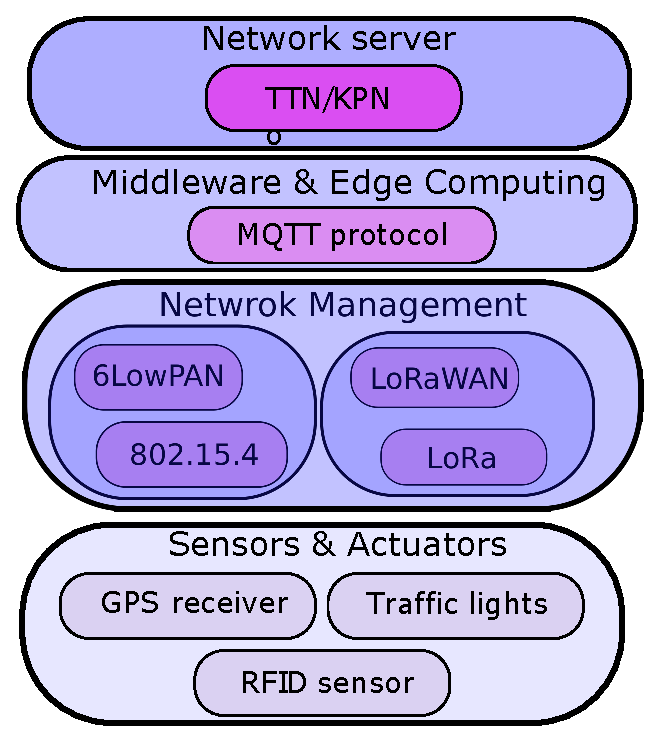
\includegraphics[width=.7\columnwidth]{architecture_loara_6lowpan}
   \flushleft
   \captionof{figure}{EES network layers}
   \label{fig:name}

    \columnbreak
    \flushleft
	\begin{tabular}{l|l|l|l}
		\bf{}               & $\ac{CF}_{[Hz]}$ & \bf{6LoWPAN} & \bf{LoRaWAN}     \\\hline
		\multirow{3}{*}{\bf{Modulation}}   & 2.4G             & O-QPSK       & -                \\
		\                                  & 915M             & BPSK         & LoRa             \\
		\                                  & 868M             & BPSK         & LoRa/GFSK        \\\hline
		\multirow{3}{*}{\bf{Channels}}     & 2.4G             & 16           & -                \\
		\                                  & 915M             & 10           & 64+8 ($\uparrow$), 8($\downarrow$)      \\
		\                                  & 868M             & 1            & 10               \\\hline
		\multirow{2}{*}{$\ac{CF}_{[MHz]}$} & 2.4G             &              & -                \\
		\                                  & 915M             & 902-929      & 902-928          \\
		\                                  & 868M             & 868-868.6    & 863-870 and 780  \\\hline
		\multirow{3}{*}{$\ac{BW}_{[Hz]}$}  & 2.4G             & 5M           & -                \\
		\                                  & 915M             & 2M           & 125K-500K        \\
		\                                  & 868M             & 600M         & 125K-250K        \\\hline
		\multirow{3}{*}{$\ac{DR}_{[bps]}$} & 2.4G             & 250M         & -                \\
		\                                  & 915M             & 40M          & 980-21.9K        \\
		% \                                  & 868M             & 20M          & LoRa: 0.3K-37.5K \\
		\                                  &                  &              & FSK:	50K         \\\hline
		\multirow{3}{*}{$\ac{CR}_{[dBm]}$} & 2.4G             & -85          & -                \\
		\                                  & 915M             & -92          &                  \\
		\                                  & 868M             & -92          & -137             \\\hline
	\end{tabular}
	\captionof{table}{LoRa and 6LowPAN characteristics \cite{al-kashoash_comparison_2016}}
	\label{tab:name}
\end{multicols}
%\bigskip

}

% \headerbox{6. Framework}{name=sea,span=2,column=1,below=screen}{

% \setlength{\columnsep}{-2.5cm}
% \begin{multicols}{2}
%     	The proposed scheme for LoRa transmission parameters selection based on GA, FL and Multi-Criteria Decision Making MCDM .
% 	\columnbreak
%     \flushright
%     % 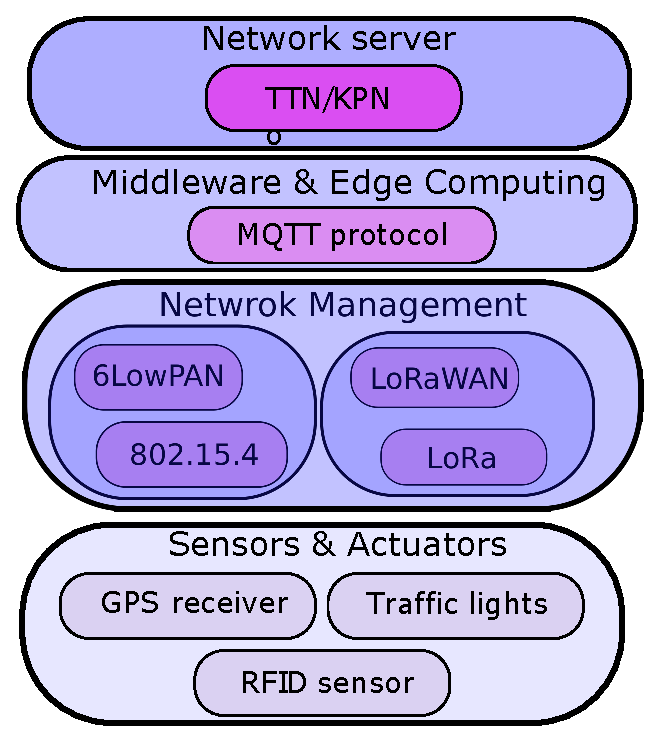
\includegraphics[width=.7\linewidth]{architecture_loara_6lowpan}
% \end{multicols}

%     \medskip
%     \Itemize{
%         \item \textbf{Ongoing:} In order to generate all the required metrics of each LoRa configuration, we use ns3 simulator with 2 nodes and one gateway. The distance between nodes and the gateway is 1km.
%     }



%     % \begin{multicols}{2}
%     %     \includegraphics[width=.8\linewidth]{generation}

%     % \columnbreak
%     %     \bigskip
%     %     \
%     %     \
%     %     \
%     %     \
%     %     \
%     %     \begin{center}
%     %     \begin{tabular}{c|c|c|c}
%     %         \textbf{Setup}   & \textbf{Selection error} & \textbf{Rank} & \textbf{Fitness} \\\hline
%     %         \textbf{1}               & 0.9                      & 1             & 1.5               \\
%     %         \textbf{2}               & 0.5                      & 3             & 4.5               \\
%     %         \textbf{3}               & 0.7                      & 2             & 3                  \\
%     %         \textbf{n}               & 0.5                      & 4             & 6                 \\
%     %     \end{tabular}
%     %     \end{center}

%     % \end{multicols}

%     % Results show that genetic algorithm select the configuration that match better the required QoS by the application.
%     % % In fact,
%     %     when we run an application that requires high quality of service,
%     %     the algorithm select the configuration that gives large BW and hight data rate with minimum enrgy consumption.
%     % When we run an application that requiers less QoS,
%     %     the algorithm rank configuration whith sufficient BW and DR.

% }

\headerbox{7. Discussion}{name=conclusion,column=1,below=screen,span=2,above=bottom}{
\bigskip
    \ding{224} \textbf{Advantages:}
To select the wireless network that best fit smart building application requirements,
	four main parameters are generally used:
	(i) cost;
	(ii) data rate;
	(iii) autonomy and (iv) communication range.
Each technology has its \ac{CF}, \ac{CR} and \ac{BW} which are compiled in the table above.

    \ding{224} \textbf{Conclusion:}
\ac{LPWAN},
	\ac{WSN} and \ac{IoT} architecture are the first candidates to ensure disaster monitoring and management systems.
	Particularly,
		IEEE802.15.4 and LoRa networks give new insight for effective \ac{EES}.
	This work gives an overview of deployment of \ac{IoT} architecture for \ac{EES}.
		Such services and demand for edge computing in real-time poses new architectural and service orchestration challenges.
	As a future work,
		we plan to study the efficiency of using a \blue{reinforcement learning} to adapt these two networks to the emergency situation of the building.
	}

\headerbox{7. References}{name=references,column=0,span=1,below=model,above=bottom}{
    \small
    \renewcommand{\section}[2]{\vskip 0.05em} 
    % \bibliographystyle{unsrt}
    \printbibliography
}
\end{poster}

